\documentclass{amsdtx}
\usepackage[margin=.75in]{geometry}
\usepackage{graphicx}
\usepackage{float}
\usepackage{eqnarray,amsmath}
\usepackage{amssymb}
\usepackage{hyperref}
\usepackage{url}
\usepackage[dvipsnames]{xcolor}
\usepackage{cancel}
\usepackage{multicol}
\usepackage[Glenn]{fncychap}
%\usepackage{hyperref}
\definecolor{b}{HTML}{3C78D8}
\definecolor{g}{HTML}{38761D}
\definecolor{r}{HTML}{AB0000}
\definecolor{p}{HTML}{A64D79}
\usepackage{textgreek}
\usepackage{listings}
\newcommand{\bs}[1]{\boldsymbol{#1}}

\definecolor{codegreen}{HTML}{38761D}
\definecolor{codeblue}{HTML}{000076}
\definecolor{codegray}{rgb}{0.2,0.2,0.2}
\definecolor{codepurple}{HTML}{AB0000}
\definecolor{backcolour}{rgb}{0.95,0.95,0.95}

\DeclareFontFamily{U}{wncy}{}
    \DeclareFontShape{U}{wncy}{m}{n}{<->wncyr10}{}
    \DeclareSymbolFont{mcy}{U}{wncy}{m}{n}
    \DeclareMathSymbol{\Sh}{\mathord}{mcy}{"58}

\lstdefinestyle{mystyle}{
    backgroundcolor=\color{white},   
    commentstyle=\color{codegreen},
    keywordstyle=\color{codepurple},
    numberstyle=\ttfamily\scriptsize\color{codeblue},
    stringstyle=\color{b},
    basicstyle=\ttfamily\footnotesize,
    breakatwhitespace=false,         
    breaklines=true,                 
    captionpos=b,                    
    keepspaces=true,                 
    numbers=left,                    
    numbersep=5pt,                  
    showspaces=false,                
    showstringspaces=false,
    showtabs=false,                  
    tabsize=4
}
\lstset{style=mystyle}

\newcolumntype{M}[1]{>{\centering\arraybackslash}m{#1}}
\newcolumntype{N}{@{}m{0pt}@{}}

\newcommand{\vfs}[1]{\ensuremath \textbf{\textit{f}}\kern-0.1cm_{s_{#1}}}
\newcommand{\fs}[1]{\ensuremath f\kern-0.07cm_{s_{#1}}}
\newcommand{\F}{\ensuremath \textbf{F}\kern-0.07cm}
\newcommand{\cc}{\ensuremath\mu_{cc}}
\newcommand{\cg}{\ensuremath\mu_{cg}}
\newcommand{\sinc}{\ensuremath\text{\kern0.06cmsinc\kern0.03cm}}
\usepackage{enumitem}

\title{\sc Apogee Detection}
\author{\sc Marc D Nichitiu | MIT Rocket Team Avionics | Project Zephyrus}
\date{\sc 26 Nov 2025}
\begin{document}
\maketitle    
\section{Abstract}
\textit{This write-up clarifies various algorithms for apogee detection for the rocket \textbf{Zephyrus}, using data from the rocket \textbf{Xanthus}. We intend to find the algorithm allowing for fastest, simplest, and most accurate apogee detection.}
\section{Proposals}
\subsection{100 Foot Drop}
The latest on-rocket implementation of apogee detection uses a 100-ft drop: barometer data is used to identify altitude, and a 100-ft drop is searched for. This method has been proven to succeed, without record of false positives and missed events. However, it relies on barometer accuracy which could become non-neglibile for higher altitudes. 
\subsection{Yaw and Pitch Angles}
Initially, we propose a measurement of the angle from the vertical,
\begin{align}
	\gamma \equiv \cos^{-1}(\cos(\psi) * \cos(\theta))
\end{align}
where $\psi$ is the yaw, and $\theta$ is the pitch ($\varphi$ is the roll angle). This calculation seems usable:~\\[-2em]
\begin{multicols}{2}
	
\begin{figure}[H]
\centering
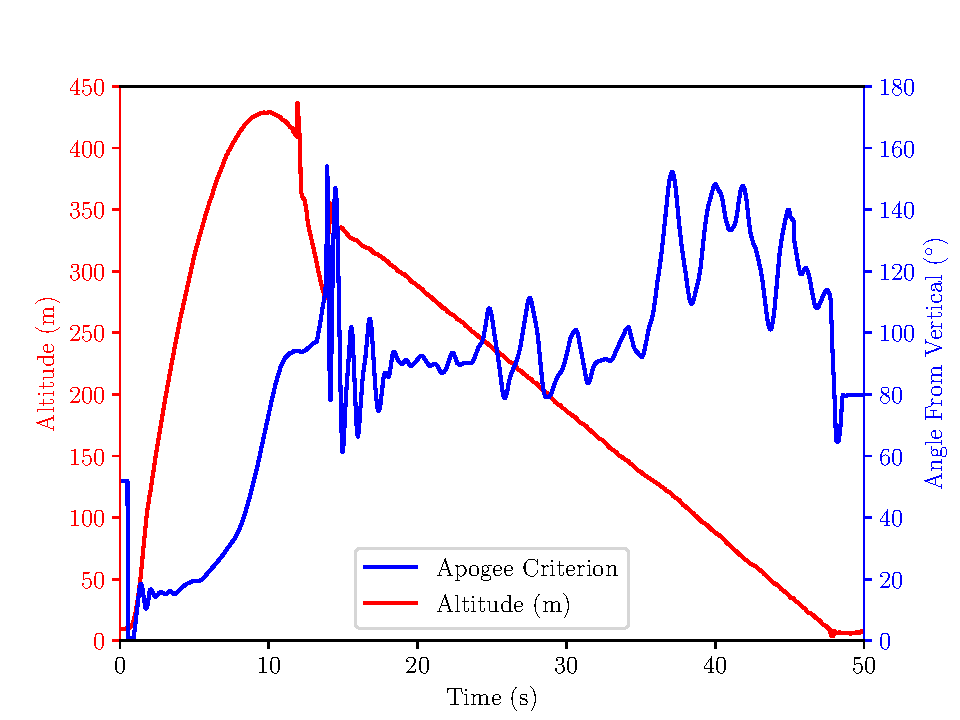
\includegraphics[width=0.5\textwidth]{fig0.pdf}	
\caption{Proposed angle-from-vertical apogee criterion in blue, for 2nd Xanthus launch data.}
\end{figure}
~\\[0.5em]We can use this to refine the apogee detection, according to the following algorithm:
\begin{verbatim}
	if (altitude > 100m) {
	    if (gamma > 45deg) {
	        if (smoothGammaDeriv < lastSmoothGammaDeriv) {
	            markApogee()   
	        }
	    }
	}
\end{verbatim}
where the smoothed $\dot\gamma$ would be calculated using a $1\rm~s$ moving average:
\begin{verbatim}
for i in range(len(gdot)):
    size = int(1/dt) + 1 # half a second
    if i < size:  
        gdotsmooth.append(gdot[i])
    else:
        gdotsmooth.append.append(np.mean(gdot[i-size:i]))
\end{verbatim}
\end{multicols}
\noindent The performance is shown on the following graph.
\begin{figure}[H]
\centering
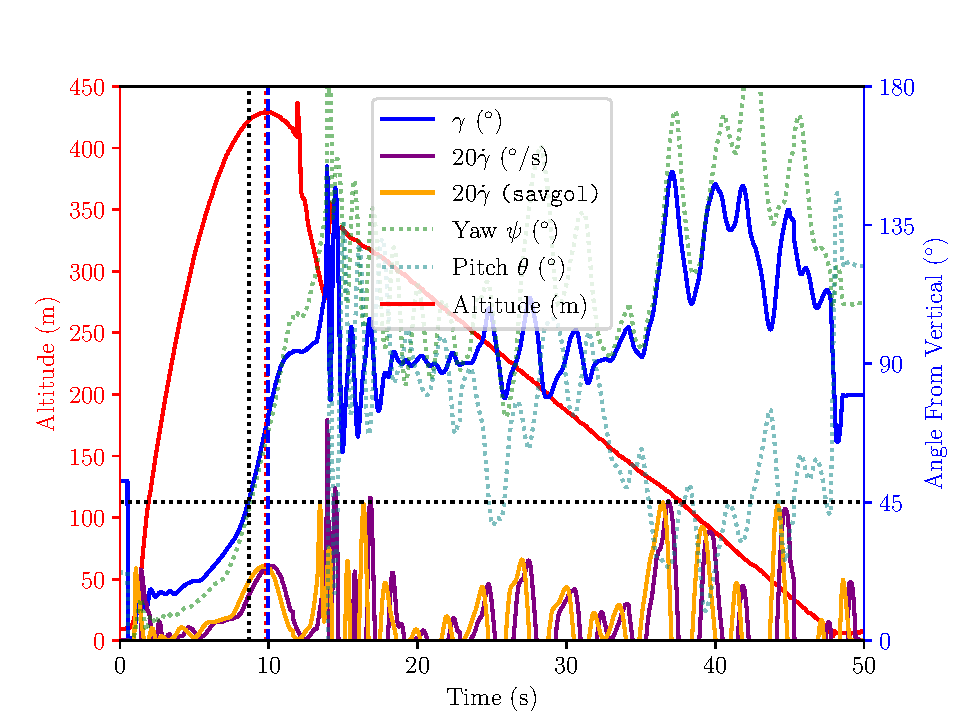
\includegraphics{fig1.pdf}	
\caption{Proposal of Apogee Detection, using the aforementioned angle. The orange line denotes a Savitzky-Golay filtered derivative, essentially a noise-free derivative to highlight accumulated lag from the moving average. In this case, the result is acceptable, and is quite close to the true apogee according to altitude.}
\end{figure}
\noindent We are able to detect apogee $\boxed{2}$ seconds earlier than the 100-ft drop, and we are able to detect apogee to within $\boxed{0.15}$ of the true altitude apogee. 
 


\end{document}





















































